\documentclass[tikz,border=8pt]{standalone}
\usetikzlibrary{arrows.meta,positioning}
\begin{document}
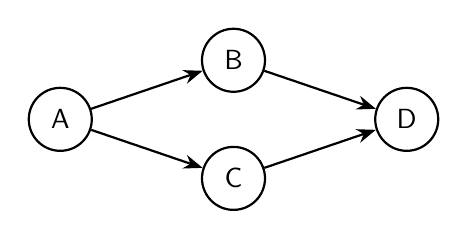
\begin{tikzpicture}[x=1cm,y=1cm]
\tikzset{
  graphnode/.style={circle,draw,thick,minimum size=8mm,inner sep=1pt,font=\sffamily},
  directed/.style={-{Stealth[length=2.4mm]},thick},
  undirected/.style={thick}
}
\node[graphnode] (n_A) at (-2.20,0.00) {A};
\node[graphnode] (n_B) at (0.00,0.75) {B};
\node[graphnode] (n_C) at (0.00,-0.75) {C};
\node[graphnode] (n_D) at (2.20,0.00) {D};
\draw[directed] (n_A) -- (n_B);
\draw[directed] (n_A) -- (n_C);
\draw[directed] (n_B) -- (n_D);
\draw[directed] (n_C) -- (n_D);
\end{tikzpicture}
\end{document}
